\subsection{Oracle RDBMS et un simple ramasse miette pour C/C++}

Il fût un temps où j'essayais d'en apprendre plus sur Oracle RDBMS, cherchais des vulnérabilités, etc.
C'est un énorme logiciel, et une fonction typique peut prendre de très larges objets
imbriqués comme arguments.
Et je voulais afficher ces objets, sous forme d'arbres (ou de graphes).

Je suivais aussi toutes les allocations/libérations de mémoire en interceptant les
fonctions d'allocation/libération.
Et lorsqu'une fonction interceptée prenait un pointeur sur un bloc de mémoire, je
cherchais ce bloc dans une liste de blocs alloués.
J'obtenais sa taille + un nom court du bloc
(ceci est comme "tagué" dans le noyau de l'OS Windows\footnote{Plus d'information
sur les commentaires dans les blocs alloués:  \CNotes{} \url{http://yurichev.com/C-book.html}}).

Pour un bloc donné, je peux le balayer à la recherche de mots 32-bit (sur les OS
32-bit) ou de mots 64-bit (sur les OS 64-bit).
Chaque mot peut être un pointeur sur un autre bloc.
Et si c'est le cas (je trouve ceci dans un autre bloc dans mes enregistrements),
je peux chercher récursivement.

\myindex{GraphViz}
Et ensuite, en utilisant GraphViz, je peux générer un tel diagramme:

\begin{figure}[H]
\centering
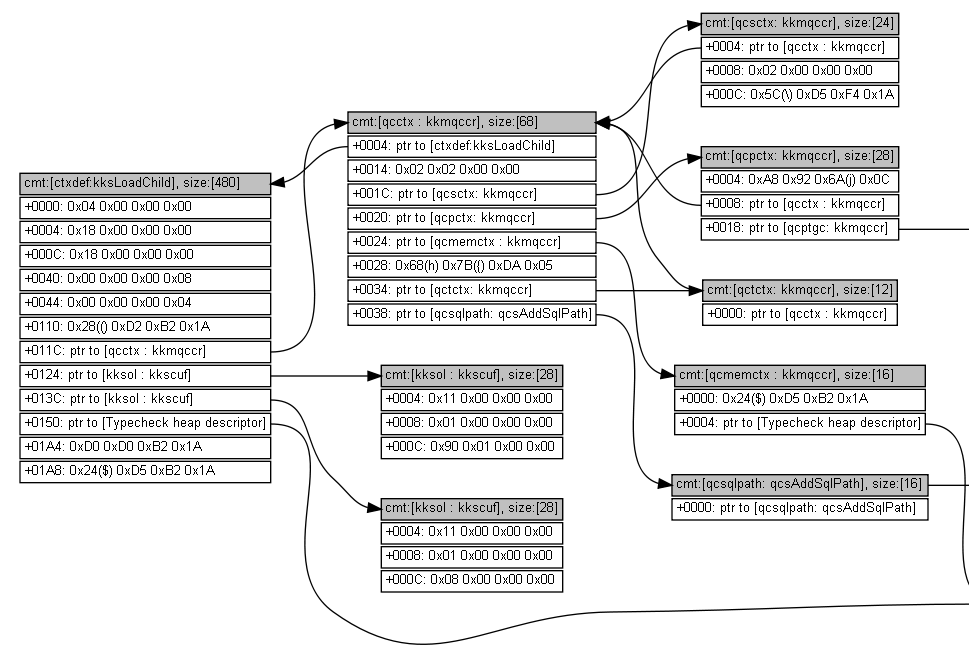
\includegraphics[scale=0.55]{advanced/450_more_ptrs/oracle2_crop.png}
\end{figure}

Images plus grosses:
\href{https://raw.githubusercontent.com/DennisYurichev/RE-for-beginners/master/advanced/450_more_ptrs/oracle1.png}{1},
\href{https://raw.githubusercontent.com/DennisYurichev/RE-for-beginners/master/advanced/450_more_ptrs/oracle2.png}{2}.

Ceci est assez impressionnant, compte tenu du fait que je n'ai aucune information
à propos des types de données de toutes ces structures.
Mais je peux en obtenir des informations.

\subsubsection{Maintenant le ramasse miette pour C/C++: Boehm GC}

\myindex{Garbage collector}
Si vous utilisez un bloc alloué en mémoire, son adresse doit être présente quelque
part, comme un pointeur dans une structure ou un tableau dans un autre bloc alloué,
ou dans une structure allouée globale, ou dans une variable locale sur la pile.
S'il n'y a plus de pointeur sur un bloc, vous pouvez l'appeler "orphelin", et il
est une cause des fuites de mémoire.

Et c'est ce qu'un \ac{GC} fait.
Il balaye tous les blocs (car il garde un \oe{}il sur tous les blocs alloués) à
la recherche de pointeurs.
Il est important de comprendre qu'il n'a aucune idée du type de données de tous les
champs de ces structures dans le blocs---ceci est important, le \ac{GC} n'a aucune information
sur les types.
Il balayage juste les blocs à la recherche de mots 32-bit ou 64-bit, et regarde s'ils
peuvent être des pointeurs sur d'autres bloc(s).
Il balaye aussi la pile.
Il traite les blocs alloués et la pile comme des tableaux de mots, dont certains pourraient
être des pointeurs.
Et s'il trouve un bloc alloué, qui est "orphelin", i.e., sur lequel aucun autre pointeur
sur lui depuis un autre bloc ou la pile, ce bloc est considéré comme inutile, devant
être libéré.
Le processus de balayage prend du temps, et c'est pourquoi les \ac{GC}s sont critiqués.

\myindex{Boehm garbage collector}
Ainsi, un \ac{GC} comme celui de Boehm\footnote{\url{https://www.hboehm.info/gc/}}
(pour du C pur) possède une fonction comme \verb|GC_malloc_atomic()|---en l'utilisant,
vous  déclarez que le bloc alloué avec cette fonction ne contiendra jamais de pointeur
vers un autre bloc.
Ça peut être une chaîne de texte, ou un autre type de donnée.
(En effet, \verb|GC_strdup()| appelle \verb|GC_malloc_atomic()|.)
Le \ac{GC} ne va pas le balayer.

% Even more: if \ac{GC}'s memory allocator thinks it can find a better place for a block, it can \emph{move} it to another place, and then fix (rewrite) all addresses,
% pointing to it, in all other blocks and in stack.
